\section{Architecture and Design}

The service has four layers:

\begin{itemize}[noitemsep, topsep=2pt]
    \item \textbf{Bootstrap} - \texttt{FileDeduplicationBootstrapImpl} is the composition root, discovered via \texttt{ServiceLoader}. It initialises all engines and wires them together.
    \item \textbf{Frontend Gate} - \texttt{FrontendGateImpl} exposes the two-method JSON API required by the frontend team (\texttt{accept} / \texttt{acceptStream}).
    \item \textbf{Deduplication engines} - \texttt{KotlinFileDeduplicator} (exact, SHA-256 + byte comparison) and \texttt{ImageFileDeduplicator} (similarity, OpenCV template matching) both implement the internal \texttt{FileDeduplicator} interface.
    \item \textbf{Storage integration} - \texttt{FileDeduplicator} extends the provided \texttt{StorageChecker} interface.
\end{itemize}

On startup, \texttt{initialize} builds an index of the entire VirtualFileSystem.

At request time, \texttt{FrontendGateImpl} selects the scan type and returns grouped results as JSON.

The Storage Team uses \texttt{findDuplicate(path)}. It first checks the existing index; if the entry is missing, it computes the hash.

\subsection{UML Class Diagram}

\begin{figure}[h!]
    \centering
    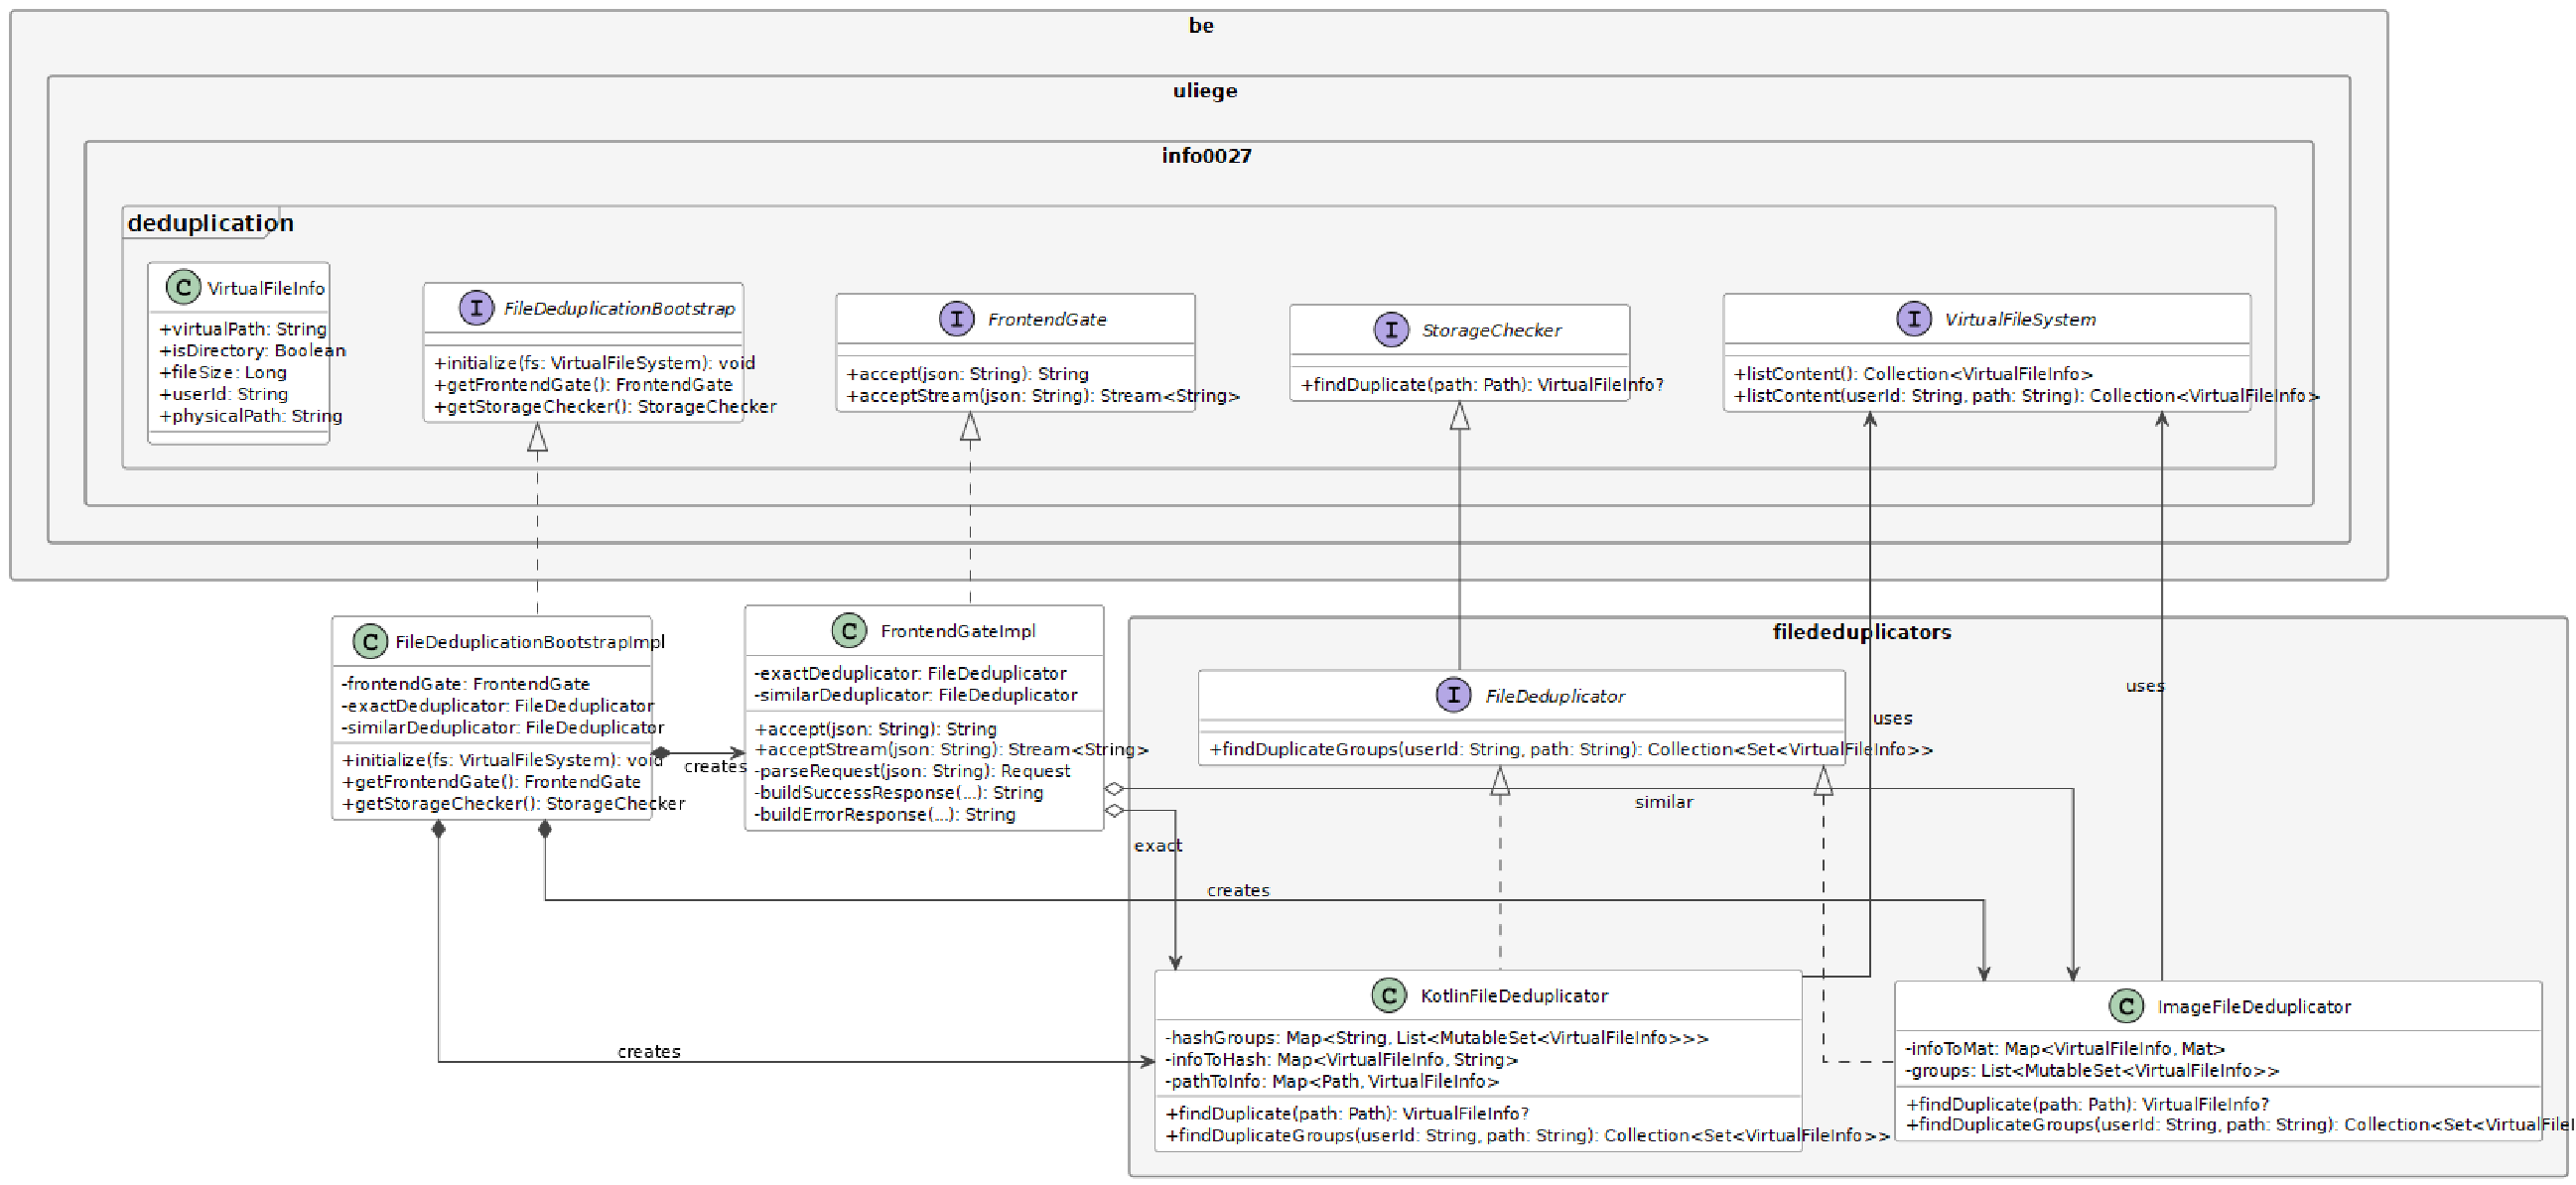
\includegraphics[width=\linewidth]{uml.pdf}
    \caption{UML Class Diagram.}
    \label{fig:uml}
\end{figure}
